\documentclass[12pt,a4paper]{report}
\usepackage[utf8x]{inputenc}
\usepackage[T1]{fontenc}
\usepackage[spanish]{babel}
\usepackage[left=1.5cm,top=2cm,right=1.5cm,bottom=2.5cm]{geometry}
\usepackage{fancyhdr}
\usepackage{graphicx}
\usepackage{float}%para poder usa argumento H en por ejemplo imagenes
\usepackage{comment}

\usepackage{titlesec}
\renewcommand{\thesection}{\arabic{section}}
\setcounter{secnumdepth}{4} %Para poner sub subsecciones (\subsubsection{<subsection>}) y para un nivel mas de subsección hay que poner \paragraph{<subsubsubsection>}
\titlelabel{\thetitle.\quad} %Para que ponga un punto desdpues de numerar una sección

\usepackage{listings}

\lstset{literate=
  {¡}{{!`}}1  {¿}{{¿`}}1
  {á}{{\'a}}1 {é}{{\'e}}1 {í}{{\'i}}1 {ó}{{\'o}}1 {ú}{{\'u}}1
  {Á}{{\'A}}1 {É}{{\'E}}1 {Í}{{\'I}}1 {Ó}{{\'O}}1 {Ú}{{\'U}}1
  {à}{{\`a}}1 {è}{{\`e}}1 {ì}{{\`i}}1 {ò}{{\`o}}1 {ù}{{\`u}}1
  {À}{{\`A}}1 {È}{{\'E}}1 {Ì}{{\`I}}1 {Ò}{{\`O}}1 {Ù}{{\`U}}1
  {ä}{{\"a}}1 {ë}{{\"e}}1 {ï}{{\"i}}1 {ö}{{\"o}}1 {ü}{{\"u}}1
  {Ä}{{\"A}}1 {Ë}{{\"E}}1 {Ï}{{\"I}}1 {Ö}{{\"O}}1 {Ü}{{\"U}}1
  {â}{{\^a}}1 {ê}{{\^e}}1 {î}{{\^i}}1 {ô}{{\^o}}1 {û}{{\^u}}1
  {Â}{{\^A}}1 {Ê}{{\^E}}1 {Î}{{\^I}}1 {Ô}{{\^O}}1 {Û}{{\^U}}1
  {œ}{{\oe}}1 {Œ}{{\OE}}1 {æ}{{\ae}}1 {Æ}{{\AE}}1 {ß}{{\ss}}1
  {ű}{{\H{u}}}1 {Ű}{{\H{U}}}1 {ő}{{\H{o}}}1 {Ő}{{\H{O}}}1
  {ç}{{\c c}}1 {Ç}{{\c C}}1 {ø}{{\o}}1 {å}{{\r a}}1 {Å}{{\r A}}1
  {€}{{\EUR}}1 {£}{{\pounds}}1
}
\lstset{extendedchars=\true,
    linewidth=\textwidth,
    inputencoding=utf8x,
    language=C++,
    xleftmargin=5pt,
    xrightmargin=5pt,
    breaklines=true,
    numberstyle=\scriptsize,
    stepnumber=1,
    numbers=left,%          Que haya números a la izquierda (número de linea)
    numbersep=5pt,
    tabsize=3,showtabs=false,
    basicstyle=\ttfamily\small,%    Estilo básico de la tipografía del código
    commentstyle=\color{Gray},%     Color de los comentarios
    showstringspaces=false,%        Los espacios no se ven de forma especial
    stringstyle=\color{BrickRed},%  Estilo de las cadenas
    keywordstyle=\color{ForestGreen},%  Estilo de las palabras reservadas
    morekeywords=[1]{size_t,ssize_t},%  Definición de más palabras reservadas
    deletekeywords={typedef,enum,do,while,if,else,for,case,default,switch,break,continue},%
        keywords=[2]{typedef,enum,do,while,if,else,for,case,default,switch,break,continue,EXIT_SUCCESS,EXIT_FAILURE},
    keywordstyle=[2]{\color{BurntOrange}},% 2do grupo de palabras reservadas
        directives={define,undef,include,if,else,ifndef,ifdef,elif,endif},%
    directivestyle=\color{NavyBlue},%       Estilo de directivas
    keywords=[3]{define,undef,include,if,else,ifndef,ifdef,elif,endif},%
    keywordstyle=[3]{\color{MidnightBlue}},%3er grupo de palabras reservadas
    morecomment=[s][\color{Gray}]{/*}{*/}%  Definición de estilo de comentario
    }  

\usepackage{color}
\definecolor{Apricot}{RGB}{253,199,130}
\definecolor{Aquamarine}{RGB}{0,181,202}
\definecolor{Bittersweet}{RGB}{192,79,23}
\definecolor{Black}{RGB}{0,0,0}
\definecolor{Blue}{RGB}{0,0,255}
\definecolor{BlueGreen}{RGB}{0,179,184}
\definecolor{BlueViolet}{RGB}{71,57,146}
\definecolor{BrickRed}{RGB}{182,50,28}
\definecolor{Brown}{RGB}{121,37,0}
\definecolor{BurntOrange}{RGB}{247,146,29}
\definecolor{CadetBlue}{RGB}{116,114,154}
\definecolor{CarnationPink}{RGB}{242,130,180}
\definecolor{Cerulean}{RGB}{0,162,227}
\definecolor{CornflowerBlue}{RGB}{65,176,228}
\definecolor{Cyan}{RGB}{0,174,239}
\definecolor{Dandelion}{RGB}{253,188,66}
\definecolor{DarkOrchid}{RGB}{164,83,138}
\definecolor{Emerald}{RGB}{0,169,157}
\definecolor{ForestGreen}{RGB}{0,155,85}
\definecolor{Fuchsia}{RGB}{140,54,140}
\definecolor{Goldenrod}{RGB}{255,223,66}
\definecolor{Gray}{RGB}{148,150,152}
\definecolor{Green}{RGB}{0,166,79}
\definecolor{GreenYellow}{RGB}{223,230,116}
\definecolor{JungleGreen}{RGB}{0,169,154}
\definecolor{Lavender}{RGB}{244,158,196}
\definecolor{LimeGreen}{RGB}{141,199,62}
\definecolor{Magenta}{RGB}{236,0,140}
\definecolor{Mahogany}{RGB}{169,52,31}
\definecolor{Maroon}{RGB}{175,50,53}
\definecolor{Melon}{RGB}{248,158,123}
\definecolor{MidnightBlue}{RGB}{0,103,149}
\definecolor{Mulberry}{RGB}{169,60,147}
\definecolor{NavyBlue}{RGB}{0,103,149}
\definecolor{OliveGreen}{RGB}{60,128,49}
\definecolor{Orange}{RGB}{245,129,55}
\definecolor{OrangeRed}{RGB}{237,19,90}
\definecolor{Orchid}{RGB}{175,114,176}
\definecolor{Peach}{RGB}{247,150,90}
\definecolor{Periwinkle}{RGB}{121,119,184}
\definecolor{PineGreen}{RGB}{0,139,114}
\definecolor{Plum}{RGB}{146,38,143}
\definecolor{ProcessBlue}{RGB}{0,176,240}
\definecolor{Purple}{RGB}{153,71,155}
\definecolor{RawSienna}{RGB}{151,64,6}
\definecolor{Red}{RGB}{237,27,35}
\definecolor{RedOrange}{RGB}{242,96,70}
\definecolor{RedViolet}{RGB}{161,36,107}
\definecolor{Rhodamine}{RGB}{239,85,159}
\definecolor{RoyalBlue}{RGB}{0,113,188}
\definecolor{RoyalPurple}{RGB}{97,63,153}
\definecolor{RubineRed}{RGB}{237,1,125}
\definecolor{Salmon}{RGB}{246,146,137}
\definecolor{SeaGreen}{RGB}{63,188,157}
\definecolor{Sepia}{RGB}{103,24,0}
\definecolor{SkyBlue}{RGB}{70,197,221}
\definecolor{SpringGreen}{RGB}{198,220,103}
\definecolor{Tan}{RGB}{218,157,118}
\definecolor{TealBlue}{RGB}{0,174,179}
\definecolor{Thistle}{RGB}{216,131,183}
\definecolor{Turquoise}{RGB}{0,180,206}
\definecolor{Violet}{RGB}{88,66,155}
\definecolor{VioletRed}{RGB}{239,88,160}
\definecolor{White}{RGB}{255,255,255}
\definecolor{WildStrawberry}{RGB}{238,41,103}
\definecolor{Yellow}{RGB}{255,242,0}
\definecolor{YellowGreen}{RGB}{152,204,112}
\definecolor{YellowOrange}{RGB}{250,162,26}

\begin{document}
	
	\begin{titlepage}

	\begin{center}

		\vspace*{0.2mm}
			\begin{figure}[htp]
				\begin{center}
					
\includegraphics[scale=1]{logo1.jpg} 
				\end{center}
			\end{figure} 

			FACULTAD DE INGENIERÍA \\
			DE LA \\
			UNIVERSIDAD DE BUENOS AIRES\\
		
		\vspace*{0.20in}
	
			\begin{Large}
				Algoritmos y Programación II [95.12]\\
			\end{Large}	
			
		\vspace*{1cm}
	
			\begin{huge}
				Trabajo Práctico n.° 1:\\
			\end{huge}
		
		\vspace*{0.75cm}
	
			\begin{Huge}
				\textbf{Objetos y algoritmos} \\
			\end{Huge}
		
		\vspace*{1.75cm}
		
		
				
			\begin{large}
				\begin{description}
					\item[\hspace{0.15 cm}Integrantes:]
						Grassi, Tomás Miguel ($99551$) - tomas96@gmail.com 					
					\item[\hspace{0.15 cm}\textcolor{white}{Integrantes:}]
						Martinez Mikulic, Mateo ($99602$) - mmartinezmikulic@gmail.com
					\item[\hspace{0.15 cm}\textcolor{white}{Integrantes:}]
						Wagner, Marcos ($98607$) - marcoswagneer.18@gmail.com
					\item[\hspace{1.4 cm}\textcolor{white}{aux}]
					\item[\hspace{0.10 cm}Profesor:]
						Ing. Calvo, Patricia
					\item[\hspace{0.10 cm}\textcolor{white}{Profesor:}]	
						Ing. Santi, Leandro
					\item[\hspace{0.10 cm}\textcolor{white}{Profesor:}]	
						Lic. Santi, Lucio
				\end{description}
			\end{large}
			
		
		\vspace*{0.8 cm}
	
		\rule{80mm}{0.1mm}\\
	
		\vspace*{0.1in}
	
			\begin{large}
				Curso 1 \\
				Jueves 17 de Mayo de 2018 \\
			\end{large}
		
	\end{center}

\end{titlepage}		

	\section{Introducción}	
		
		\indent En este trabajo se busca obtener conocimientos de programación orientada a objetos y de diseño de algoritmos. Para ello se
		realiza un programa utilizando el patrón de diseño Strategy y se mejora el diseño original previo de la transformada discreta de Fourier
		implementando la transformación rápida de Fourier (FFT) y su transformada inversa (IFFT).
		
	\section{Diseño e implementación del programa}	
	
        \subsection{Diseño del programa}
            \indent Se implementó para este programa la clase Complex y la clase Vector, ambas implementadas como templates.
            De esta forma se logra una mayor simplicidad, ya que se codifica una única función sin importar el tipo de dato que
            se le pase como parámetro, logrando un código más mantenible. Además, a partir del uso del uso de templates se logra una
            generalización de cada clase, ya que la misma se puede utilizar para distintos tipos de datos. Por ejemplo, la clase vector,
            gracias a la implementación en forma de plantilla, es posible que cada instancia del vector contenga cualquier objeto, como
            un complejo, o tipo de dato que se necesite. 
            \\
            \indent La clase Complex es utilizada para cargar cada uno de los datos leídos y dentro de la clase Vector se ordenan en
            orden leído cada uno de los objetos de la clase Complex. 
   			\\
			\indent Para la clase Complex se sobrecargaron los operadores correspondientes a la suma, resta, multiplicación, 
			división, los cuales son utilizados en la implementación de todas las transformadas. Además se sobrecargaron los operadores
			de asignación, negación y comparación. De esta forma se logra un código más mantenible y legible. Por otro lado para 
			la clase vector se sobrecargaron los operadores de asignación e indexación. 
			\\
			\indent Por último, se utilizó el código provisto para el manejo de argumentos,	realizando los cambios necesarios para que 
			parsee el archivo de señales, de forma que lea una señal por línea.

		\subsection{Patrón de diseño}
			
			\begin{figure}[H]
				\centering
					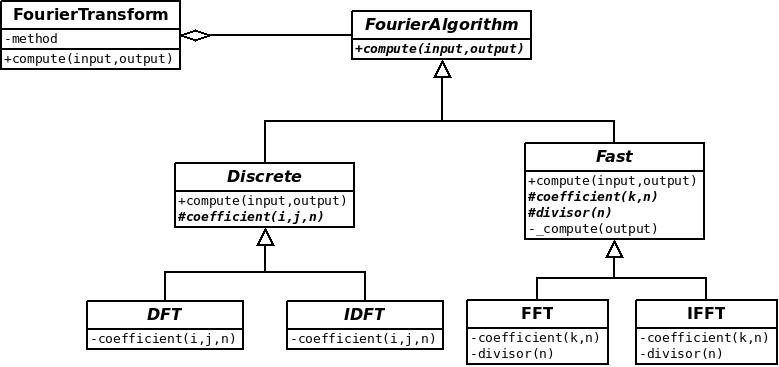
\includegraphics[scale=0.55]{diagrama_de_clases.jpg}
				\caption{Diagrama de clases según el lenguaje unificado de modelado UML}
			\end{figure}
			

			\indent Se utilizó para este proyecto el patrón de diseño Strategy. Esto permite reutilizar código y proporciona
			al usuario una misma interfaz que asegura un correcto funcionamiento sin importar la transformada utilizada. Según
			el método elegido el constructor de FourierTransform recibirá un puntero a una subclase de FourierAlgorithm. Esta subclase de FourierAlgorithm ejecutará la función \textit{\_compute()} con el coeficiente correspondiente.

		\subsection{Diseño del algoritmo de la transformada rápida de Fourier}
			\indent La transformada rápida de Fourier se realizó de manera recursiva con el método dividir y conquistar, aprovechando 
			la propiedad de las raíces complejas de la unidad y su periodicidad, que permite computar la DFT en tiempo \textit{O(nlg(n))},
			en lugar de \textit{O(n²)}. El requisito para esto es que el número de entradas sea una potencia de 2. Al realizar dividir
			y conquistar se divide en cada pasada recursiva a los elementos en posiciones par y a los posicionados en numeros impares, 
			y se los procesa por separado, logrando reducir la cantidad de operaciones totales.   


		\subsection{Interfaz}

			\indent La interacción con el programa es a través de comandos en línea de ordenes. Tanto la entrada 
			como la salida, puede direccionarse desde o hacia un archivo utilizando el flag correspondiente (\textit{-i, -o}
			respectivamente) seguido del nombre del archivo. En caso de no indicar ningún archivo, el programa utiliza los 
			flujos standar de entrada (por teclado) y salida (por pantalla). Por otro lado, también es posible indicar el método 
			de transformación que se desea utilizar a partir del flag de método \textit{-m} e indicando luego el método por su
			abreviatura (DFT, IDFT, FFT o IFFT). En caso de que esta opción no sea indicada, el programa realiza la FFT por defecto.

		\subsection{Formato de entrada y salida}

			\indent El archivo de entrada será un archivo de texto con pares ordenados de complejos (re, im), separados por
			espacios. Cada línea en el archivo de entrada será una señal diferente. La salida tendrá el mismo formato, siendo 
			cada línea la transformada o antitransformada de la señal correspondiente. 


	\section{Corridas de prueba}
	 
		\indent Las pruebas realizadas son similares a las realizadas en el proyecto anterior. Solo se agregaron las pruebas 
		correspondientes al procesamiento de datos con FFT e IFFT. Estas pruebas permitieron determinar que el tiempo de 
		procesamiento de la transformada rápida de Fourier es mil veces mas rápida que la transformada discreta de Fourier. 
		\\
		\indent En las pruebas realizadas con un número de entradas diferente a una potencia de dos el resultado varía al 
		desarrollado por la DFT al rellenar con ceros los complejos faltantes.
		\\	
		\indent Para realizar las pruebas de funcionamiento decidimos usar Google C++ Testing Framework, una herramienta que 
		permite que las pruebas sean independientes y repetibles. Permite separar las pruebas en módulos separados, reflejando 
		la estructura del código evaluado y logrando de esta manera que sea mas entendible y mantenible. Al fallar una prueba, 
		según la naturaleza de la falla, la prueba puede seguir desarrollándose o simplemente detener ese módulo para continuar 
		con el siguiente. 	
		\\
		\indent En este proyecto se realizaron pruebas sobre las clases desarrolladas y luego sobre el procesamiento de datos.
		Al realizar pruebas sobre las clases se verificó que las funciones correspondientes a la clase Complex funcionaran 
		correctamente, tomando como patrón de comparación la clase \textit{std::complex} definida en el archivo de cabecera
		\textit{<complex.h>} provisto por la biblioteca estándar de C++. Al desarrollar las pruebas de procesamiento de datos 
		el enfoque fue primero la verificación del correcto funcionamiento tanto de la función \textit{DFT()} como de la 
		función \textit{IDFT()} y luego la robustez del proceso, realizando pruebas que variaban en el volumen de datos 
		pseudo-aleatorios obtenidos con \textit{rand()}.
		\\
		\indent Asimismo, se realizaron pruebas para determinar cuál debía ser el valor máximo en que pueden diferir dos números
		para ser considerados iguales. Para esto se fueron ejecutando las pruebas creadas para números complejos y para la DFT variando,
		de a potencias de diez, el factor por el que se multiplicaba a \textit{std::numeric\_limits<long double>::epsilon()}, el cual es
		la diferencia mínima que debe	haber	entre 1 y un número para que éste sea considerado el siguiente valor respresentable. 
		De esta forma se llegó a una cota en el valor mínimo de comparación: $10^{-6}$.
		\\
		\indent Para ejecutar las pruebas sólo es necesario usar el comando make y luego ejecutar el programa de pruebas;
		éstas informan si alguno de los resultados no es el esperado.


	\section{Problemas durante el desarrollo y soluciones}
		
        \indent Al realizar el algoritmo de un proceso tan complejo como la transformada rápida de Fourier se desarrollaron varios
        problemas y contratiempos hasta que se pudo lograr una versión del algoritmo funcional. Estos errores fueron causados por el
        uso de la recursividad en un algoritmo del cual desconocíamos su funcionamiento. Los valores en el exponente en \textit{coefficient()} 
        y el desarrollo de la función inversa fue lo que más confusión causó.
        \\
        \indent Por otro lado, utilizando Valgrind se verificó que no hubiera fuga de memoria. Inicialmente había un uso incorrecto de
        memoria dinámica lo cual provocó que el programa pise memoria que no le correspondia. Gracias a este diagnóstico se pudo diseñar 
        el programa de forma correcta.

   

	\section{Conclusiones}
	
		\indent	El programa cumple su función de manera eficaz cualquiera sea el método de la transformada que se utilice. La eficiencia
		del mismo depende del método utilizado, siendo la FFT mil veces más eficiente que la DFT en cuanto al tiempo de ejecución. Sin
		embargo, es posible mejorar ligeramente	la eficiencia del algoritmo utilizando propiedades de los numeros complejos para reducir
		parcialmente la cantidad de operaciones que se	realizan aunque la complejidad final seguiría siendo \textit{O(nlg(n))}. Por otro 
		lado utilizando algoritmos más complejos, sería posible	trabajar con una cantidad de muestras de señales que no sean
		necesariamente potencia de dos, y de esta manera evitar aproximar los resultados de nuestra transformada al completar la muestra 
		con ceros al final del vector hasta llegar a la potencia entera de 2 más cercana.
		\\
		\indent Por otro lado, utilizar herramientas como Google C++ Testing Framework facilita la tarea de probar el funcionamiento y permite
		de manera sencilla verificar el	funcionamiento a medida que diferentes cambios son realizados al código.

	\section{Bibliografía}
		
		\begin{itemize}
		\item Ghezzi, Carlo \& Jazayeri, Mehdi \& Mandrioli, Dino (1991). \textit{Fundamentals of Software Engineering} ($1.^{era}$ ed.) Upper Saddle River, NJ 07458: Prentice Hall, Inc.
		\item Stroustrup, Bjarne  (1988). \textit{The C++ Programming Language}  ($4.^{ta}$ ed.) Upper Saddle River, NJ 07458: Addison-Wesley.
		\item Cormen, Thomas \& Leiserson, Charles \& Rivest, Ronald \& Stein, Clifford (1989). \textit{Introduction to Algorithms} ($1.^{era}$ ed.) Upper Saddle River, NJ 07458: MIT Press.
		\end{itemize}

	\section{Script de compilación}
	
		makefile
		\lstinputlisting[frame=single]{makefile}
				
	\section{Código fuente}
	
		main.h
		\lstinputlisting[frame=single]{main.h}

   		main.cpp
		\lstinputlisting[frame=single]{main.cpp}

		cmdline.h
		\lstinputlisting[frame=single]{cmdline.h}
		
		cmdline.cpp
		\lstinputlisting[frame=single]{cmdline.cpp}		
		
		io.h
		\lstinputlisting[frame=single]{io.h}

		io.cpp
		\lstinputlisting[frame=single]{io.cpp}

		fourier.h
		\lstinputlisting[frame=single]{fourier.h}
		
		fourier.cpp
		\lstinputlisting[frame=single]{fourier.cpp}
						
		Vector.h
		\lstinputlisting[frame=single]{Vector.h}
		
		Complex.h
		\lstinputlisting[frame=single]{Complex.h}

		fourier\_test.h
		\lstinputlisting[frame=single]{fourier_test.h}

		fourier\_test.cpp
		\lstinputlisting[frame=single]{fourier_test.cpp}

		Complex\_test.h
		\lstinputlisting[frame=single]{Complex_test.h}

		Complex\_test.cpp
		\lstinputlisting[frame=single]{Complex_test.cpp}

		
		
	

\end{document}